\begin{frame}
  \frametitle{Hybrid $S_N$-Diffusion Method: Proposed Work}
  \begin{block}{\textbf{Development of a Hybrid $S_N$-Diffusion Method for Control Rod Modeling}}
    \textbf{Sub-objectives}
    \begin{enumerate}
      \item Development \& Implementation of the Hybrid Method in Moltres
        \begin{itemize}
          \item Implementation in Moltres
          \item SVDC Calculation
          \item Correction Region Size
          \item Autonomous Buffer Zone Determination
        \end{itemize}
      \item Verification of the Hybrid Method
      \item Computational Performance Characterization of the Hybrid Method
        \begin{itemize}
          \item Relative speedup vs. $S_N$ method
          \item Scaling performance
        \end{itemize}
      \item Demonstration of the Hybrid Method for Transient Analysis
    \end{enumerate}
  \end{block}
\end{frame}

\begin{frame}
  \frametitle{Hybrid $S_N$-Diffusion Method: Proposed Work}
  \textbf{Sub-objective 1: Development \& Implementation of the Hybrid Method in Moltres}
  \vspace{.2cm}

  \textbf{Implementation:}
  \begin{itemize}
    \item 3-D $S_N$ solver with a diffusion synthetic acceleration scheme
    \item Extend the existing neutron diffusion solver to accept diffusion coefficient vectors
    \item Automate multigroup $S_N$-diffusion coupling through the MOOSE MultiApp and Action
      systems
    \item Supporting features (e.g., SVDC calculations, buffer zone calculations)
  \end{itemize}
\end{frame}

\begin{frame}
  \frametitle{Hybrid $S_N$-Diffusion Method: Proposed Work}
  \textbf{Sub-objective 1: Development \& Implementation of the Hybrid Method in Moltres}
  \vspace{.2cm}

  \textbf{\gls{SVDC} Calculation}

  The existing formulation for SVDCs are undefined at flux peaks and troughs:
  \begin{align}
    D^s_g(x) &= -J^{tr}_g(x)\bigg/\frac{d\phi^{tr}_g(x)}{dx} \nonumber
  \end{align}
  I will explore alternative formulations to avoid division by the flux gradient. For instance,
  Tomatis \& Dall'Osso \cite{tomatis_application_2011} developed the following formulation for
  additive corrections for the Ronen method:
  \begin{align}
    \delta D(x_{i+1/2},E) =& -\delta J(x_{i+1/2},E) \frac{(\Delta x_{i+1}+\Delta x_i)/2}{
    \phi(x_{i+1},E)+\phi(x_i,E)}
    \shortintertext{where}
    x_i =& \mbox{ $i$-th spatial interval,} \nonumber \\
    \delta J(x,E) =& J_{tr}(x,E) - J_D(x,E), \nonumber \\
    \Delta x_i =& \mbox{ size of $i$-th spatial interval.} \nonumber
  \end{align}
\end{frame}

\begin{frame}
  \frametitle{Hybrid $S_N$-Diffusion Method: Proposed Work}
  \textbf{Sub-objective 1: Development \& Implementation of the Hybrid Method in Moltres}
  \vspace{.2cm}
  
  \textbf{Correction Region Size}
  \vspace{.1cm}

  The correction region represents the problem domain of the $S_N$ sub-solver.
  \vspace{.2cm}
  
  I will investigate 2-D and 3-D problems derived from the MSRE design to create a set of criteria
  for the minimum required correction region size. My preliminary work showed that the:
  \begin{itemize}
    \item geometrical heterogeneity and
    \item optical thickness
  \end{itemize}
  strongly influence the \gls{SVDC} and the minimum correction region size.
\end{frame}

\begin{frame}
  \frametitle{Hybrid $S_N$-Diffusion Method: Proposed Work}
  \textbf{Sub-objective 1: Development \& Implementation the Hybrid Method in Moltres}
  \vspace{.2cm}

  \textbf{Autonomous Buffer Zone Determination}
  \vspace{.1cm}

  \begin{columns}
    \column{.6\textwidth}
    %For the 1-D problems, I set up an outward-sweeping algorithm that compares \glspl{SVDC} with the
    %default $P_1$-based diffusion coefficients.
    %The algorithm terminates when the coefficient values
    %coincide, beyond which the hybrid method reverts to the $P_1$-based coefficients (buffer zone).
    The outward-sweeping algorithm for determining the buffer zone is more ambiguous for 2-D and
    3-D geometries which contain more than one coordinate axis.
    \vspace{.2cm}

    I will investigate 2-D and 3-D problems to analyze \gls{SVDC} distributions and identify
    helpful patterns for developing an algorithm for autonomous buffer zone determination.
    \column{.4\textwidth}
    \begin{figure}
      \centering
      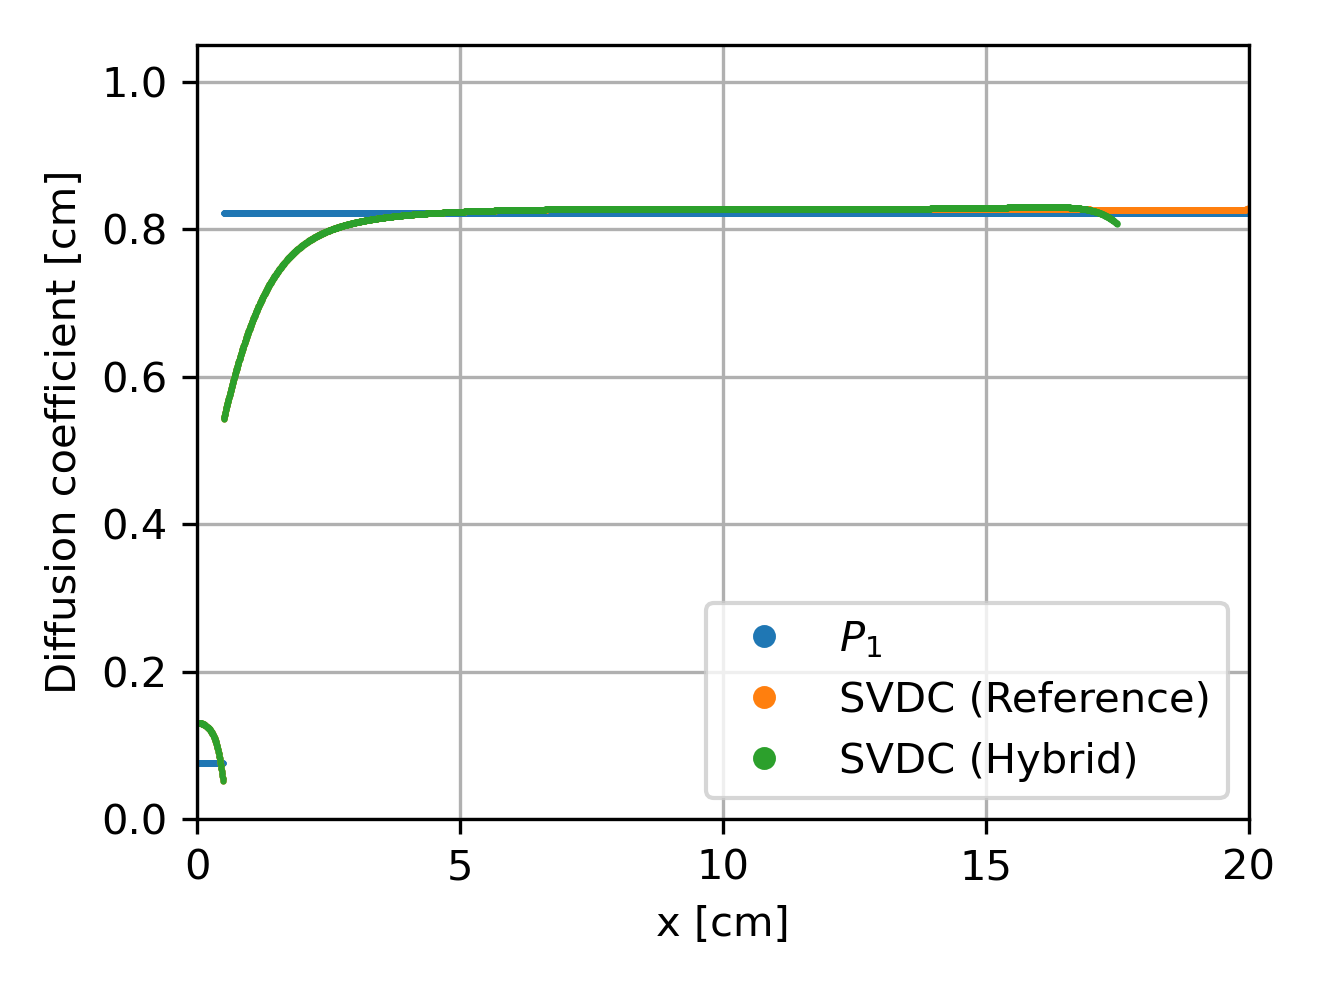
\includegraphics[width=\textwidth]{../images/case-0-group-2-hybrid-diffcoef}
      \caption{Diffusion coefficients for group 2 flux in Case 0.}
    \end{figure}
  \end{columns}
\end{frame}

\begin{frame}
  \frametitle{Hybrid $S_N$-Diffusion Method: Proposed Work}
  \textbf{Sub-objective 2: Verification of the Hybrid Method}
  \vspace{.2cm}

  \begin{columns}
    \column{.65\textwidth}
    I will verify the hybrid method against reference OpenMC calculations of several test cases,
    leading up to a 3-D model of the MSRE. The verification study
    will include permutations of the following factors:
    \begin{itemize}
      \item 2-D and 3-D models derived from the MSRE model
      \item Asymmetric control rod positions
      \item Control rods at various levels of insertion
    \end{itemize}
    \column{.35\textwidth}
    \begin{figure}
      \centering
      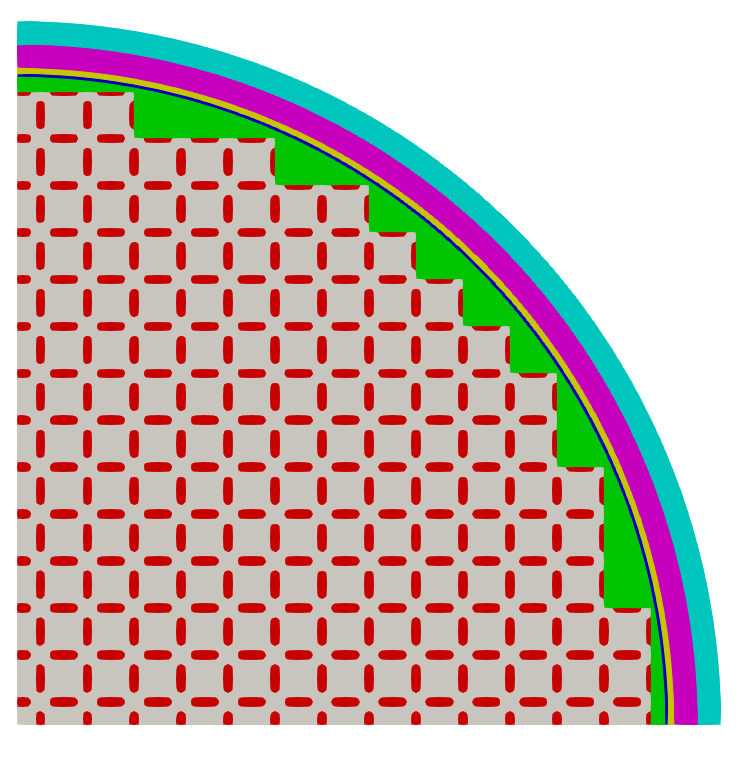
\includegraphics[width=\textwidth]{images/msre-slice}
      \caption{Horizontal cross section view of the MSRE.}
    \end{figure}
  \end{columns}
\end{frame}

\begin{frame}
  \frametitle{Hybrid $S_N$-Diffusion Method: Proposed Work}
  \textbf{Sub-objective 3: Characterize the computational performance of the hybrid method}
  \vspace{.2cm}

  The hybrid method is expected to be significantly faster than the standard $S_N$ method due to:
  \begin{itemize}
    \item the small correction region size relative to the full reactor geometry
    \item faster convergence of SVDCs compared to neutron flux in $S_N$ calculations
  \end{itemize}
  I will conduct performance characterization on the 2-D and 3-D verification study models for the
  following factors:
  \begin{itemize}
    \item Speedup relative to the standard $S_N$ method
    \item Slowdown relative to the standard neutron diffusion method
    \item Weak and strong scaling on computing clusters
  \end{itemize}
\end{frame}

\begin{frame}
  \frametitle{Hybrid $S_N$-Diffusion Method: Proposed Work}
  \textbf{Sub-objective 4: Demonstration of the Hybrid Method for Transient Analysis}
  \vspace{.2cm}

  The ultimate goal of developing the hybrid method is to enable transient analyses involving
  moving control rods with Moltres.
  \vspace{.2cm}

  I will demonstrate multiphysics simulations of control rod insertion and ejection transients
  on 2-D and 3-D models with the hybrid method.
\end{frame}
